\documentclass{Thesis-TE-ITS}

\title{Buku Thesis Teknik Elektro ITS}
\author{John Doe}
\date{July 2019}

\begin{document}

\begin{abstract}
This is a simple paragraph at the beginning of the 
document. A brief introduction about the main subject.
\end{abstract}

\chapter{PENDAHULUAN}\label{Bab 1}

\section{Latar belakang}
Sint voluptate est dolor proident. Irure exercitation incididunt ullamco eiusmod duis esse ad deserunt est mollit Lorem eiusmod aliqua cillum. Eiusmod ullamco consectetur ad esse cillum cupidatat sunt occaecat laborum officia irure eu minim. Quis laboris sint esse elit. Exercitation minim veniam aute consequat culpa culpa laborum exercitation fugiat nostrud. Reprehenderit reprehenderit eiusmod amet duis commodo est aute elit mollit amet et sunt duis.

\begin{figure}[h]
    \centering
    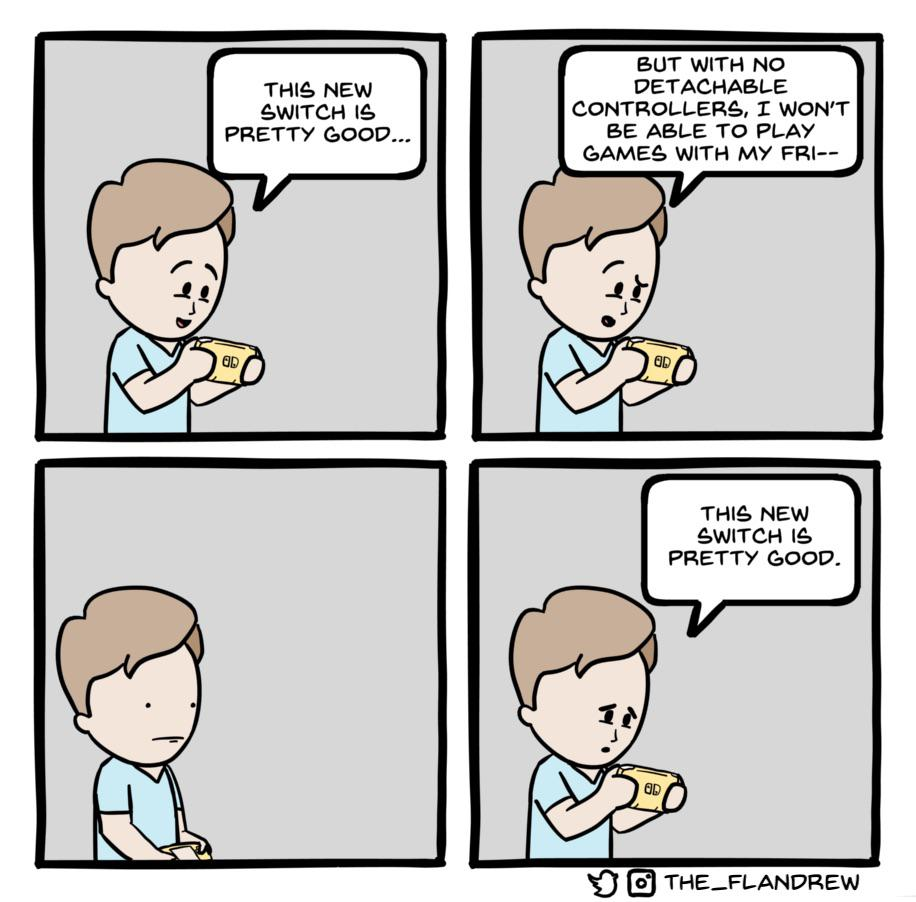
\includegraphics[width=0.25\textwidth]{images/meme.jpg}
    \caption{a nice plot}
    \label{fig:mesh1}
\end{figure}

As you can see in the figure \ref{fig:mesh1}

\begin{itemize}
\item The individual entries are indicated with a black dot, a so-called bullet.
\item The text in the entries may be of any length.
\end{itemize}

\begin{enumerate}
\item This is the first entry in our list
\item The list numbers increase with each entry we add
\end{enumerate}

The mass-energy equivalence is described by the \ref{gambar:meme1} famous equation
\[E=mc^2\]
discovered in 1905 by Albert Einstein. 
In natural units ($c = 1$), the formula expresses the identity

\begin{equation}
E=m
\end{equation}

\gambar
    {images/meme.jpg}
    {this is a caption}
    {meme1}
    {0.5}

\chapter{PENDAHULUAN}

\section{Latar Belakang}

Latar belakang menyajikan konteks penelitian, untuk apa penelitian ini dilakukan, dan hal apa yang mengarahkan penelitian ini. Disini diuraikan dalam keadaan bagaimana topik akan dilakukan.

Latar belakang memuat studi awal atau berbagai teori utama yang relevan dan baru (\emph{recent}) yang dipadukan sehingga mengerucut pada suatu persoalan unik yang kemudian disusun dalam bentuk perumusan masalah. Lazimnya bagian ini diawali dengan menguraikan kesenjangan, teoritik, maupun praktis, antara harapan dan kenyataan.

\section{Rumusan Masalah}

Dalam sub-bab ini, permasalahan yang ingin diselesaikan dirumuskan secara jelas, tajam, dan terfokus. Bagian ini memuat uraian/pernyataan atau berbagai topik pokok yang akan digali dalam penelitian ini. Definisi, asumsi, dan lingkup penelitian/studi dapat pula dijelaskan pada bagian ini. Perumusan masalah menyebutkan fokus utama dari penelitian yang mencakup berbagai pertanyaan yang akan dijawab dalam penelitian sehingga gambaran tentang apa yang akan diungkapkan dalam penelitian perlu terurai dengan jelas. Semua pertanyaan yang diajukan perlu didukung oleh alasan perlandas/dasar yang diperoleh dari studi awal atau teori utama.

\section{Tujuan}

Pada bagian ini, tujuan dilakukannya penelitian tesis dan target atau sasaran yang ingin dicapai dinyatakan secara singkat dan jelas sesuai dengan permasalahan yang telah dirumuskan. Penelitian tesis dapat bertujuan untuk menjajaki, menguraikan, menjelaskan, membuktikan, atau menerapkan suatu konsep/hipotesa/gejala, atau membuat suatu prototip.

\section{Batasan Masalah}

Batasan masalah diperlukan bila penelitian tesis terlalu luas sehingga perlu dilakukan batasan-batasan dalam penyelesaian permasalahan dalam penelitian. Batasan juga dapat berupa batasan fisik sistem bila tesis membahas implementasi metode pada sistem real.

\section{Kontribusi}
Kontribusi yang diharapkan dari hasil penelitian tesis terkait dengan tujuan penelitian.

\end{document}